\chapter{基于 Transformer 的两阶段横向移动检测方法}{
{
\let\cleardoublepage\relax
}

根据本文第~\ref{chap:analyze}~章和第~\ref{chap:embedding}~章的分析,攻击者发起横向移动攻击之后,将使得一部分横向移动流量在批量传输特征、数据包长度特征等的值超出了良性流量相应的值域,并且使网络的拓扑结构发生更改,这反映了攻击者利用被攻破的负载与集群的 API 服务器进行非法通信等行为。此外,还有大多数横向移动流量仍然十分隐蔽,不能通过特征分析和拓扑分析直接进行分类。

因此,本文将分别针对这两类横向移动流量进行研究,并提出基于 Transformer 的两阶段横向移动检测方法。该方法应能:

\begin{itemize}
    \item 检出关键横向移动流量,这些横向移动流量体现出横向移动的关键行为;
    \item 对于大多数横向移动流量,应在误报率较低的水平上尽可能提高检测率,AUC 分数达到 95\% 以上,优于其他现有的模型。
\end{itemize}

本章将提出基于 Transformer 的两阶段横向移动检测方法。在第一阶段,基于最值和拓扑的横向移动检测方法负责检测关键的横向移动流量;在第二阶段,基于 Transformer 的横向移动检测模型 LMDCE 检测大多数横向移动流量,由空间特征嵌入模块、时间特征嵌入模块、编码器—解码器模块和两阶段预测机制构成,以提高模型的性能。本文通过实验,验证了方法的有效性,并且其性能高于已有的方法。

\section{问题定义}

本文考虑的横向移动检测是一个自监督的问题。给定时间连续的两个流量序列
\begin{equation}
    \label{eq:definition}
    \begin{split}
        \tau_1 &= \left \langle X_1, X_2, \cdots, X_t \right \rangle ,\\
        \tau_2 &= \left \langle X_{t+1}, X_{t+2}, \cdots, X_T \right \rangle ,
    \end{split}
\end{equation}
在假设 $\tau_1$ 为良性流量序列的情况下,需对未知序列 $\tau_2$ 中的每个流量 $X_i$ 进行二分类,分类结果为该流量是良性流量,或该流量是横向移动流量。

其中,每个流量 $X_i$ 由源节点 $s_i$、目的节点 $d_i$ 和流量特征 $\mathbf{x}_i$ 组成。

\section{总体流程}

方法的总体流程如图~\ref{fig:total-model}~所示。

\begin{figure}[t]
    \centering
    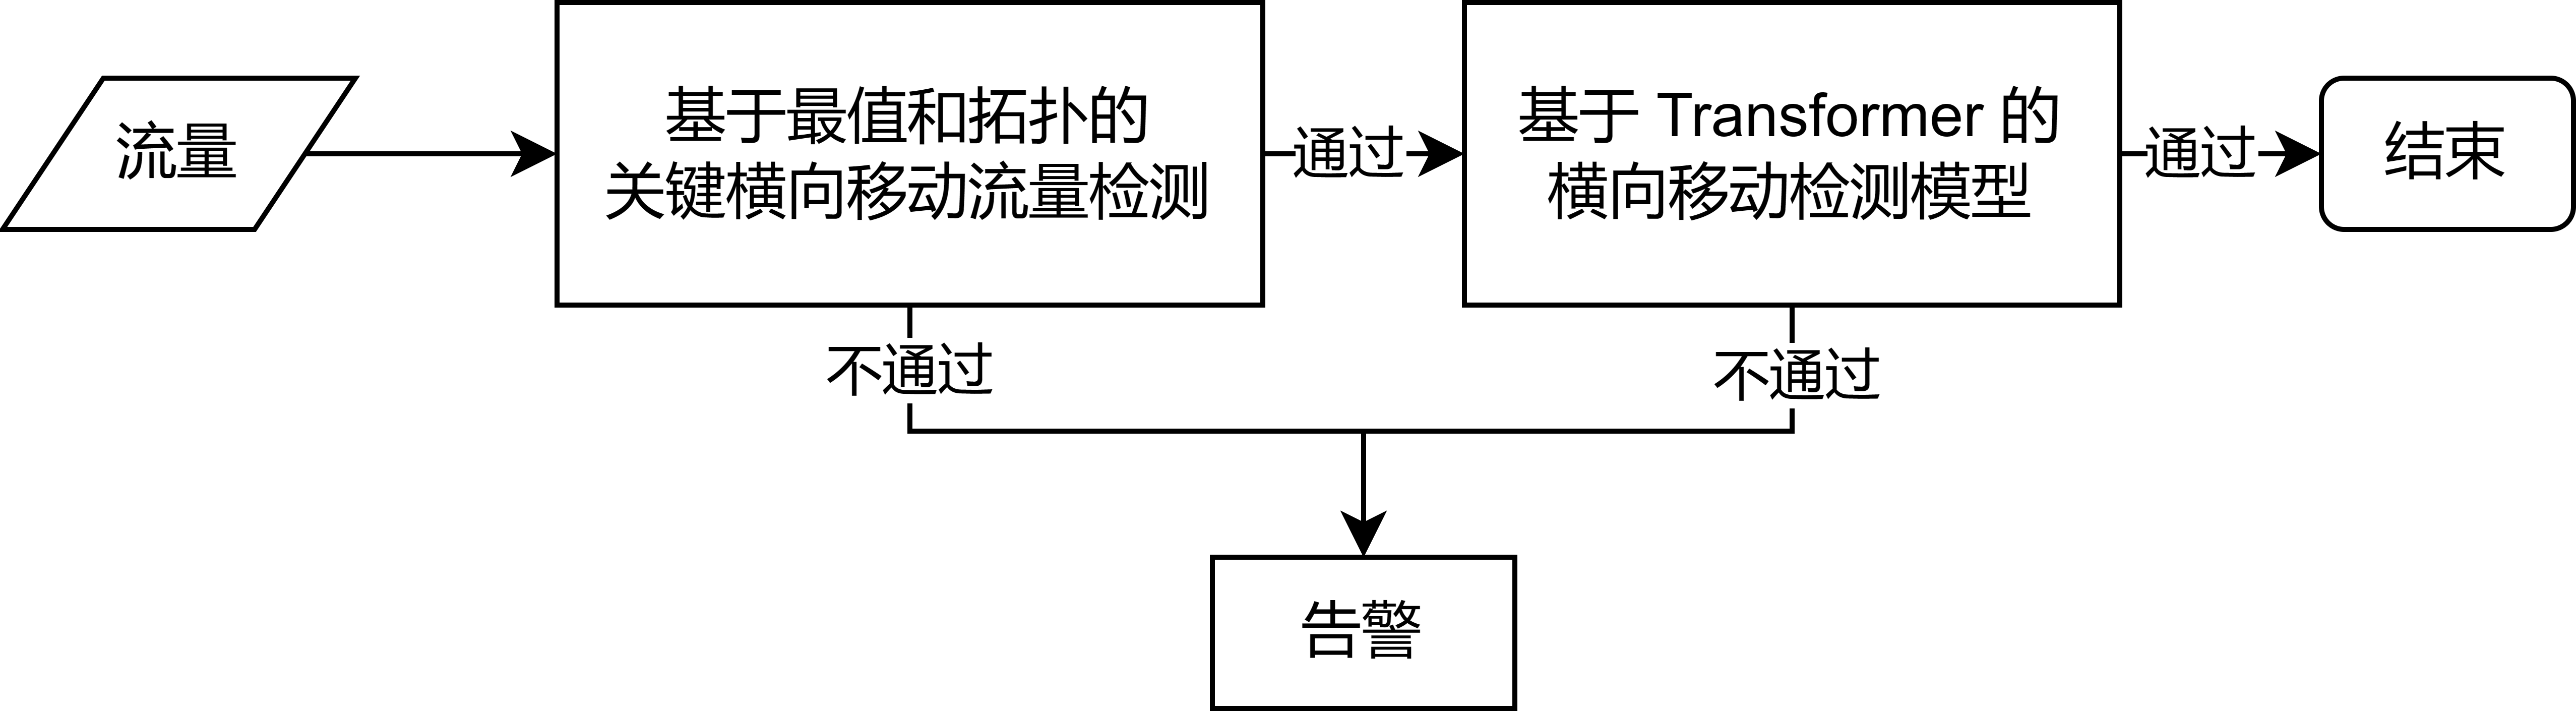
\includegraphics[width=0.75\textwidth]{total-model}
    \bicaption{\enspace 基于 Transformer 的两阶段横向移动检测方法总体流程}{\enspace The overall workflow of the lateral movement detection method based on Transformer}
    \label{fig:total-model}

\end{figure}

流量按时间顺序逐个输入。按照本研究的目标,方法将由两阶段构成。

为了检出关键的横向移动流量,方法首先将根据最值和拓扑对流量进行检测,未能通过检测(即被识别为横向移动)的流量将发出告警;通过检测的大部分流量,再由基于 Transformer 的横向移动检测模型进行检测,未能通过检测的流量将发出告警,通过检测的流量视为正常流量。

将方法分为两个阶段进行设计有两个好处:

\begin{itemize}
    \item 提高了可解释性。基于最值和拓扑的检测方法具有很强的可解释性,该方法可以明确指出横向移动流量的哪些特征超出了正常范围,或它导致网络流量拓扑发生了哪些改变;而基于 Transformer 等深度学习的模型具有不可解释性\citep{SAEED2023110273}。
    \item 提高了横向移动流量的检测率。基于 Transformer 的横向移动检测模型进行检测可以检出绝大多数的横向移动流量,是高检测率的支柱;而基于最值和拓扑的检测方法可以进一步检出前述模型尚不能检出的横向移动流量,是该模型的补充,可进一步提高检测率。
\end{itemize}

\section{第一阶段:基于最值和拓扑的横向移动检测}

本节将利用第~\ref{sec:extreme}~节和第~\ref{sec:topology}~节的分析结果,对横向移动流量进行检测。

\subsection{基于最值的横向移动流量检测}

根据第~\ref{sec:extreme}~节的最值分析,横向移动将改变容器化集群中的网络流量模式,使连续活跃时长最大值等特征的值超过了良性流量的相应值。因此,本文提出了基于最值的横向移动流量检测方法。该方法分为两个阶段进行:

\begin{itemize}
    \item 训练阶段。在该阶段,读入网络流量,更新网络流量特征的最值。
    \item 检测阶段。在该阶段,读入网络流量,并判断其各项特征是否超出了最值,超出的判定为横向移动。
\end{itemize}

该方法使用的特征包括前向数据包长度最大值、前向每 bulk 传输字节数、前向每 bulk 传输数据包数、前向 bulk 速率、连续活跃时长最大值。这些特征的有关分析见第~\ref{sec:extreme}~节。

方法的伪代码如图~\ref{fig:detect-code}~所示。

\begin{figure}[t]
    \centering
    \begin{subfigure}[b]{1.0\textwidth}
        \hrulefill
        \begin{algorithmic}[1]
            \Require $\tau_1$, FeatureList
            \Ensure MinMap, MaxMap
            \Function {TrainMap}{$\tau_1$, FeatureList}
                \State MinMap $\gets \emptyset$, MaxMap $\gets \emptyset$
                \For{$X$ \textbf{in} $\tau_1$}
                    \For{Feature \textbf{in} FeatureList}
                        \State MinMap[Feature] $\gets $ Min (MinMap[Feature], $X$[Feature])
                        \State MaxMap[Feature] $\gets $ Max (MinMap[Feature], $X$[Feature])
                    \EndFor
                \EndFor
            \EndFunction
            \end{algorithmic}
        \hrulefill
        \caption{训练阶段}
    \end{subfigure}
    \\
    \begin{subfigure}[b]{1.0\textwidth}
        \hrulefill
            \begin{algorithmic}[1]
            \Require $\tau_2$, FeatureList, MinMap, MaxMap
            \Ensure Alerts
            \Function{TestFlow1}{$\tau_2$, FeatureList, MinMap, MaxMap}
                \For{$X$ \textbf{in} $\tau_2$}
                    \For{Feature \textbf{in} FeatureList}
                        \If{$X$[Feature] $\notin$ [MinMap[Feature],MaxMap[Feature]]}
                            \State \textbf{alert} $X$
                        \EndIf
                    \EndFor
                \EndFor
            \EndFunction
            \end{algorithmic}
        \hrulefill
        \caption{检测阶段}
    \end{subfigure}
    \bicaption{\enspace 基于最值的横向移动流检测伪代码}{\enspace Pseudocode of detecting lateral movements based on min and max values}
    \label{fig:detect-code}
\end{figure}

\subsection{基于拓扑的横向移动流量检测}
\label{sec:detect-on-topology}

根据第~\ref{sec:topology}~节的拓扑分析,横向移动将改变容器化集群中的拓扑结构。本文检测以下拓扑结构的变更:

\begin{itemize}
    \item 负载节点增加;
    \item 与 API 服务器通信的节点增加,或从未与 API 服务器通信的节点开始通信;
    \item 从未访问外部网络的负载节点开始访问外部网络。
\end{itemize}

方法的伪代码如图~\ref{fig:detect-topology-code}~所示。

\begin{figure}[t]
    \centering
    \begin{subfigure}[b]{1.0\textwidth}
        \hrulefill
        \begin{algorithmic}[1]
            \Require $\tau_1$, ApiServer
            \Ensure PodSet, ApiSet, PodExternalSet
            \Function {TrainSet}{$\tau_1$, ApiServer}
                \State PodSet $\gets \emptyset$, ApiSet $\gets \emptyset$, PodExternalSet $\gets \emptyset$
                \For{$X$ \textbf{in} $\tau_1$}
                    \State $s, d \gets X$
                    \State Append $s$ to PodSet if $s$ is a Pod
                    \State Append $d$ to PodSet if $d$ is a Pod
                    \State Append $s$ to ApiSet if $d$ equals ApiServer
                    \State Append $d$ to ApiSet if $s$ equals ApiServer
                    \State Append $s$ to PodExternalSet if $s$ is a Pod and $d$ is an external node
                    \State Append $d$ to PodExternalSet if $d$ is a Pod and $s$ is an external node
                \EndFor
            \EndFunction
            \end{algorithmic}
        \hrulefill
        \caption{训练阶段}
    \end{subfigure}
    \\
    \begin{subfigure}[b]{1.0\textwidth}
        \hrulefill
            \begin{algorithmic}[1]
            \Require $\tau_2$, ApiServer, PodSet, ApiSet, PodExternalSet
            \Ensure Alerts
            \Function{TestFlow2}{$\tau_2$, ApiServer, PodSet, ApiSet, PodExternalSet}
                \For{$X$ \textbf{in} $\tau_2$}
                    \State $s, d \gets X$
                    \State malicious $\gets 0$
                    \State Set malicious to 1 if $s \notin$ PodSet and $s$ is a Pod
                    \State Set malicious to 1 if $d \notin$ PodSet and $d$ is a Pod
                    \State Set malicious to 1 if $s \notin$ ApiSet and $d$ equals ApiServer
                    \State Set malicious to 1 if $d \notin$ ApiSet and $s$ equals ApiServer
                    \State Set malicious to 1 if $s \notin$ PodExternalSet and $s$ is a Pod and $d$ is an external node
                    \State Set malicious to 1 if $d \notin$ PodExternalSet and $d$ is a Pod and $s$ is an external node
                    \If{malicious $= 1$}
                        \State \textbf{alert} $X$
                    \EndIf
                \EndFor
            \EndFunction
            \end{algorithmic}
        \hrulefill
        \caption{检测阶段}
    \end{subfigure}
    \bicaption{\enspace 基于拓扑结构的横向移动流检测伪代码}{\enspace Pseudocode of detecting lateral movements based on topology}
    \label{fig:detect-topology-code}
\end{figure}

\section{第二阶段:LMDCE,基于 Transformer 的横向移动检测模型}

对于大部分横向移动流量,其检测的难点在于:它们隐蔽在正常流量之间,无法直接利用它们的特征判别出来。特别是,经过了基于最值和拓扑的检测之后,横向移动流量就更加隐蔽了。尽管本文已经提取了这些流量的空间嵌入向量和时间嵌入向量,但是,还需要有效的深度学习模型才能进行检测。

因此,本文提出了基于 Transformer 的横向移动检测模型,并称其为 LMDCE(Lateral Movement Detection in Containerized Environments)。LMDCE 的结构如图~\ref{fig:model}~所示。

\begin{figure}[t]
    \centering
    \includegraphics[width=1.00\textwidth]{model}
    \bicaption{\enspace LMDCE 模型结构}{\enspace The architecutre of LMDCE}
    \label{fig:model}

\end{figure}

LMDCE 是基于预测的横向移动检测模型。LMDCE 分为空间特征嵌入模块、时间特征嵌入模块、编码器—解码器模块和两步预测机制。

\subsection{空间特征嵌入模块}

LMDCE 采用 GCN 作为空间特征嵌入方法,如第~\ref{sec:spatial}~节所述。

考虑到在基于拓扑的横向移动流量检测中,包含有新负载的流量已经被识别为横向移动流量,因此,在 LMDCE 中,可以将网络流量拓扑图视为静态的。因此,本模块独立进行训练,输入训练流量序列 $\tau_1$ 后,经过训练,为 $\tau_1$ 的每个节点生成嵌入向量。

在测试流量序列 $\tau_2$ 中,可能包含 $\tau_1$ 中所没有的新节点,因此需要考虑这些节点的嵌入向量。根据容器化集群网络结构(图~\ref{fig:networking}),新节点可能是新的服务、新的负载、新的主机或新的外部节点。新的主机需要容器化集群的管理员来配置,因此由攻击者创建的可能性较低,不纳入 LMDCE 的考虑范围。新的服务依赖于新的负载,而新的负载在第~\ref{sec:detect-on-topology}~节就已被筛除,因此不纳入 LMDCE 的考虑范围。所以,在 $\tau_2$ 中包含的节点只可能是新的外部节点。对于新的外部节点,本模块随机生成向量作为该节点的嵌入向量。

\subsection{时间特征嵌入模块}
\label{sec:temporal-module}

LMDCE 采用三层 LSTM 作为时间特征嵌入方法,如第~\ref{sec:temporal}~节所述。

在 LMDCE 中,时间特征嵌入模块的输出为时间特征嵌入向量,作为后续编码器—解码器模块的输入,用于自注意力机制。因此,本模块将与编码器—解码器模块一起进行训练和测试。

在自注意力机制中,时间特征嵌入向量的作用是让模型根据当前时间的特征,从编码器输出的隐向量中获取与当前特征最有关联性的信息,有助于模型生成预测,降低良性流量的预测误差,从而降低模型的误报率。

\subsection{编码器—解码器模块}

LMDCE 的编码器—解码器受 Transformer\citep{vaswani2017attention} 启发进行设计。它接收一个长度为 $n$ 的流量窗口 $W=\left<X_{t-n},\cdots,X_{t-1}\right>$ 和时间特征嵌入向量,输出该窗口下一个时刻的流量预测 $\hat{X}_t$。其中流量 $X_i$ 由源节点 $s_i$ 所对应的嵌入向量 $\mathbf{s}_i$、目的节点 $d_i$ 所对应的嵌入向量 $\mathbf{d}_i$ 和流量特征 $\mathbf{x}_i$ 连接而成。

流量窗口经过位置编码后输入到编码器中。通过多头注意力机制,编码器可以并行地处理流量窗口,计算流量之间的相关性和依赖关系\citep{vaswani2017attention}。通过前馈网络,编码器可以学习到更复杂的语义关系。最终,编码器生成隐向量。

隐向量和时间特征嵌入向量输入至解码器中。通过多头注意力机制,编码器可以并行地检索时间特征嵌入向量与流量窗口之间的相关性。编码器将根据时间特征嵌入向量,查询流量窗口中最相关的流量,随后经过输出层,得到当前流量窗口的预测。

\subsection{两步预测机制}

LMDCE 的两步预测机制受 USAD\citep{audibert2020usad}、TranAD\citep{tuli2022tranad} 的启发进行设计,但进行了改进,以进一步提高性能。

由于生成对抗网络和对抗训练机制存在不稳定性和收敛困难等问题\citep{darban2022deep,kodali2017convergence},通常不适合在线使用。因此,本文没有像以往的工作\citep{audibert2020usad, tuli2022tranad, li2019mad}那样采用对抗训练的方式,而是采用一种两步预测的方式来提升模型的性能。LMDCE 使用了一个编码器和两个解码器用于两步预测。

在第一步,模型使用编码器和第一个解码器预测流量 $X_t$,预测值为 $O_1$。随后,LMDCE 将计算 $O_1$ 与 $X_t$ 的误差,得到误差向量 $E$。

在第二步,将 $E$ 与流量窗口 $W$ 连接,再次输入至 LMDCE 的编码器中。此时,编码器中与误差向量相接的神经元将会激活,自注意力机制将更关注第一次预测中存在误差的部分。LMDCE 使用同一个编码器和第二个解码器预测流量 $X_t$,预测值为 $O_2$。

通过将误差向量重新输入至模型中,LMDCE 对良性流量的预测更准确,有助于降低误报率。

\subsection{LMDCE 的训练过程}

LMDCE 的时间特征嵌入模块单独进行训练,训练过程参见第~\ref{sec:temporal-module}~节。训练完成后,得到网络流量各节点对应的嵌入向量。

对于训练流量序列 $\tau_1$ 中的每个流量 $X_t$,取 $X_t$ 之前(不含)长度为 $n$ 的流量序列作为流量窗口 $W_t$。模型接收 $W_t$ 作为输入,输出两个预测值 $O_{1,t}$ 和 $O_{2,t}$。本文分别计算这两个预测值与实际值 $X_t$ 的误差
\begin{equation}
    \label{eq:loss}
    \begin{split}
        l_{1,t} &= \left\Vert O_1 - X_t \right\Vert,\\
        l_{2,t} &= \left\Vert O_2 - X_t \right\Vert,
    \end{split}
\end{equation}
随后,将误差加权平均,得到
\begin{equation}
    \label{eq:total-loss}
    \begin{split}
        l_t &= \epsilon l_{1,t} + (1-\epsilon)l_{2,t} ,
    \end{split}
\end{equation}
其中 $\epsilon$ 随着训练的迭代而减小。上述 $l_t$ 即是用于模型训练的损失函数。

在训练刚开始时,LMDCE 更关注流量窗口和流量整体,使预测在总体上接近实际值;随着训练迭代过程的推进,LMDCE 更关注预测存在误差的部分,使预测尽可能地接近实际值。通过这种方式,减少了良性流量的预测误差;而横向移动流量由于 LMDCE 未对其进行适配,预测的误差较大,使其容易被检测出来。

\subsection{LMDCE 的检测过程}

对于测试流量序列 $\tau_2$,检测时,LMDCE 使用 $l_{2,t}$ 作为流量 $X_t$ 的评估分数。$l_{2,t}$ 体现的是 LMDCE 经过两步预测形成的最终误差,它可以将良性流量的预测误差最小化,从而横向移动流量的预测误差变得相对较大,降低误报率,提高检测率。

在根据评估分数进行最终的分类时,还需确定异常分数的阈值。这通常可根据对误报的容忍度、对检测灵敏度的需求等动态选定。本文第~\ref{sec:threshold}~节将通过实验结果讨论阈值选定方法。

\section{实验验证}

\subsection{实验配置}
本章使用 PyTorch 进行建模、训练和测试等工作。实验的具体配置如表 \ref{tab:experiment-environment} 所示。

\begin{table}[t]
    \bicaption{\enspace 实验配置}{\enspace Experiment environment}
    \label{tab:experiment-environment}
    \centering
    \footnotesize% fontsize
    \setlength{\tabcolsep}{4pt}% column separation
    \renewcommand{\arraystretch}{1.2}%row space 
    \begin{tabular}{lcccccccc}
        \hline
        操作系统 & Ubuntu 20.04.6 LTS\\
        Python 版本 & 3.7.16\\
        Pytorch 版本 & 1.13.1\\
        CUDA 版本 & 11.7\\
        显卡 & NVIDIA RTX A60000\\
        处理器 & Intel(R) Xeon(R) Silver 4214 CPU @ 2.20GHz\\
        \hline
    \end{tabular}
\end{table}

\subsection{实验所采用的数据集}
\label{sec:experiment-dataset}

实验采用了 Kubernetes-dataset 作为数据集,数据集的详细介绍见第~\ref{sec:dataset}~节。在该数据集中,良性流量和横向移动流量是分开录制的,因此本实验将横向移动流量注入至良性流量的末尾,同时保留横向移动流量之间和良性流量之间的时间关系,并对齐了横向移动流量和良性流量的结束时间。随后,本文划分了训练集和测试集,其中训练集 $\tau_1$ 占 70\% 的网络流量,测试集 $\tau_2$ 占 30\% 的网络流量,并且所有横向移动流量仅出现在 $\tau_2$ 中。

\subsection{评估指标}
\label{sec:kpi}
混淆矩阵是评估机器学习分类模型的工具。它包含如下四个部分:

\begin{enumerate}
    \item TP(True Positive):将横向移动流正确地识别为横向移动流的样本数量。
    \item FP(False Positive):将良性流错误地识别为横向移动流的样本数量。
    \item TN(True Negative):将良性流正确地识别为良性流的样本数量。
    \item FN(False Negative):将横向移动流错误地识别为良性流的样本数量。
\end{enumerate}

基于混淆矩阵,延伸出分类模型的评价指标:真正率(召回率)、假正率、准确率、精确率、F1 分数,其定义如下:

\begin{itemize}
    \item 真正率(True Positive Rate,TPR):$\mathrm{TPR}=\frac{\mathrm{TP}}{\mathrm{TP}+\mathrm{FN}}$,代表在所有横向移动流中被检测出来的比例,在本文中也称检测率。检测率越高,代表模型的性能越好。
    \item 假正率(False Positive Rate,FPR):$\mathrm{FPR}=\frac{\mathrm{FP}}{\mathrm{FP}+\mathrm{TN}}$,代表在所有良性流中被误判为横向移动流的比例,在本文中也称误报率。误报率越低,代表模型的性能越好。
    \item 准确率(Accuracy,A):$\mathrm{A}=\frac{\mathrm{TP}+\mathrm{TN}}{\mathrm{TP}+\mathrm{FP}+\mathrm{TN}+\mathrm{FN}}$,代表在所有样本中分类正确的比例。准确率越高,代表模型的性能越好。
    \item 精确率(Precision,P):$\mathrm{P}=\frac{\mathrm{TP}}{\mathrm{TP}+\mathrm{FP}}$,代表在检出为横向移动流的样本中,实际也是横向移动流的比例。精确率越高,代表模型的性能越好。
    \item 召回率(Recall,R):$\mathrm{R}=\mathrm{TPR}$,与真正率相同。
    \item F1 分数(F1):$\frac{2\mathrm{P}\mathrm{R}}{\mathrm{P}+\mathrm{R}}$,是精确率和召回率的调和平均值。精确率和召回率往往呈负相关,F1 分数以单一指标平衡了这两个指标。
\end{itemize}

在基于异常检测的分类模型中,模型为每个样本评估位于$\left[0,1\right]$之间的异常分数,并根据一个阈值$\delta\in\left[0,1\right]$,将异常分数小于$\delta$的样本分类为正常样本,将异常分数大于$\delta$的样本分类为异常样本。将阈值$\delta$遍历$\left[0,1\right]$,可得到一系列的混淆矩阵,基于这些混淆矩阵,可以提出 ROC 曲线作为一个评估工具:

\begin{itemize}
    \item 受试者操作特征曲线(Receiver Operating Characteristic,ROC):以 FPR 为横坐标,TPR 为纵坐标作出的曲线。ROC 曲线下的面积(Area Under the Curve,AUC)越大,代表模型的性能越好。
\end{itemize}

\subsection{第一阶段方法验证与优化}
\label{sec:verify-1}

本小节将验证基于最值和拓扑的横向移动检测方法。

通过基于最值的横向移动检测方法,检出了 5 个横向移动流量,另有 3 个良性流量被误报为横向移动。这些流量的详细情况如表~\ref{tab:experiment-minmax}~所示。

\begin{table}[t]
    \bicaption{\enspace 被基于最值的横向移动检测方法检出的流量}{\enspace Flows detected by method based on min and max values}
    \label{tab:experiment-minmax}
    \centering
    \footnotesize% fontsize
    \setlength{\tabcolsep}{4pt}% column separation
    \renewcommand{\arraystretch}{1.2}%row space 
    \begin{tabular}{ccccp{4cm}cccc}
        \hline
        源 IP 地址 & 源端口 & 目的 IP 地址 & 目的端口 & 被检特征\centering & 是否为横向移动流量\\
        \hline
        144.122.71.18 & 6443 & 10.16.0.4 & 52536 & 连续活跃时长最大值\centering & 否\\
        10.16.0.4 & 46958 & 144.122.171.91 & 53 & 连续活跃时长最大值\centering & 否\\
        10.16.0.5 & 36757 & 144.122.172.92 & 53 & 连续活跃时长最大值\centering & 否\\
        10.16.0.45 & 54902 & 144.122.71.36 & 9001 & 连续活跃时长最大值、前向数据包长度最大值、前向每 bulk 传输字节数、前向 bulk 速率\centering & 是\\
        10.16.0.45 & 52904 & 144.122.71.18 & 6443 & 前向数据包长度最大值、前向每 bulk 传输字节数、前向每 bulk 传输数据包数、前向 bulk 速率\centering & 是\\
        10.16.0.45 & 52906 & 144.122.71.18 & 6443 & 前向数据包长度最大值、前向每 bulk 传输字节数、前向每 bulk 传输数据包数、前向 bulk 速率\centering & 是\\
        10.16.0.45 & 45956 & 144.122.71.18 & 6443 & 前向每 bulk 传输字节数、前向 bulk 速率\centering & 是\\
        10.16.0.45 & 47002 & 144.122.71.18 & 6443 & 前向每 bulk 传输数据包数、前向 bulk 速率\centering & 是\\
        \hline
    \end{tabular}
\end{table}

通过实验结果可以发现,``连续活跃时长最大值''特征导致了误报,而且该特征对检测作用不大,为优化检测方法,可以将此特征从基于最值的方法的特征列表中删除。

通过基于拓扑的横向移动检测方法,检出了 8 个横向移动流量,没有产生误报。除了已被最值方法检出的流量以外,其余流量的详细情况如表~\ref{tab:experiment-topology}~所示。

\begin{table}[t]
    \bicaption{\enspace 被基于拓扑的横向移动检测方法检出的流量}{\enspace Flows detected by method based on topology}
    \label{tab:experiment-topology}
    \centering
    \footnotesize% fontsize
    \setlength{\tabcolsep}{4pt}% column separation
    \renewcommand{\arraystretch}{1.2}%row space 
    \begin{tabular}{ccccccccc}
        \hline
        源 IP 地址 & 源端口 & 目的 IP 地址 & 目的端口 & 被检指标 & 是否为横向移动流量\\
        \hline
        10.16.0.45 & 54902 & 144.122.71.36 & 9001 & 新负载、与外部连接 & 是\\
        144.122.71.36 & 9001 & 10.16.0.45 & 48754 & 新负载、与外部连接 & 是\\
        10.16.0.45 & 52904 & 144.122.71.18 & 6443 & 新负载、与 API 服务器连接 & 是\\
        10.16.0.45 & 52906 & 144.122.71.18 & 6443 & 新负载、与 API 服务器连接 & 是\\
        10.16.0.45 & 59624 & 95.179.254.105 & 443 & 新负载、与外部连接 & 是\\
        10.16.0.45 & 45956 & 144.122.71.18 & 6443 & 新负载、与 API 服务器连接 & 是\\
        10.16.0.45 & 46988 & 144.122.71.18 & 6443 & 新负载、与 API 服务器连接 & 是\\
        10.16.0.45 & 47002 & 144.122.71.18 & 6443 & 新负载、与 API 服务器连接 & 是\\
        \hline
    \end{tabular}
\end{table}

实验结果表明,通过基于最值和拓扑的横向移动检测方法,可以发现关键的横向移动行为,去除重复后共有 8 条流量。攻击者在网络中创建了新的负载节点,并且该负载节点同时与 API 服务器和外部网络保持通信。

\subsection{第二阶段模型 LMDCE 的验证}
\label{sec:verify-2}

本节将 LMDCE 的性能,同时与横向移动检测模型 Euler\citep{king2023euler}、Bowman 等人\citep{bowman2020detecting},图链路预测模型 TGN\citep{rossi2020temporal},以及时间序列异常检测模型 USAD\citep{audibert2020usad}、OmniAnomaly\citep{su2019robust}、TranAD\citep{tuli2022tranad}进行对比。其中,Euler、Bowman 等人、TranAD 由本文作者重新实现;OmniAnomaly、USAD 使用了由文献\citep{tuli2022tranad}实现的版本;TGN 使用原作者的开源版本,其解码器由链路预测更改为边特征的预测(实验结果表明,链路预测的性能表现较低)。模型参数如表~\ref{tab:experiment-compare}~所示。

\begin{table}[t]
    \bicaption{\enspace 模型的训练参数}{\enspace Training parameters of models}
    \label{tab:experiment-compare}
    \centering
    \footnotesize% fontsize
    \setlength{\tabcolsep}{4pt}% column separation
    \renewcommand{\arraystretch}{1.2}%row space 
    \begin{tabular}{lp{8cm}}
        \hline
        模型 & 参数\\
        \hline
        Bowman 等人 & walk=Node2Vec(walk\_length=10, context\_size=2, p=1, q=1e-9, walks\_per\_node=20)\\
        Euler & delta=5(seconds), gnn=GCN(), rnn=GRU(n\_layers=3)\\
        TGN & batch\_size=5\\
        USAD & n\_hidden=74, n\_latent=38, n\_window=180\\
        OmniAnomaly & beta=0.01, n\_hidden=74, n\_latent=38, rnn=GRU(n\_layers=2)\\
        TranAD & n\_window=180, rnn=LSTM(num\_layers=3), gnn=GCN()\\
        LMDCE & n\_window=180, rnn=LSTM(num\_layers=3), gnn=GCN()\\
        \hline
    \end{tabular}
\end{table}

实验结果如表~\ref{tab:experiment-compare-result}~所示。

\begin{table}[t]
    \bicaption{\enspace 模型性能对比实验结果}{\enspace Comparison results}
    \label{tab:experiment-compare-result}
    \centering
    \footnotesize% fontsize
    \setlength{\tabcolsep}{4pt}% column separation
    \renewcommand{\arraystretch}{1.2}%row space 
    \begin{tabular}{ccccccccc}
        \hline
        模型 & TPR & FPR & F1 & AUC & 训练用时(秒)\\
        \hline
        Bowman 等人 & 0.0491 & 0.0004 & 0.0920 & 0.6976 & 7.2\\
        Euler & 0.5521 & 0.2633 & 0.1839 & 0.7242 & 266.1\\
        TGN & 0.6970 & 0.3013 & 0.1582 & 0.7728 & 5037.6\\
        USAD & 0.7607 & 0.3028 & 0.0930 & 0.8141 & 5953.0\\
        OmniAnomaly & 0.7485 & 0.3034 & 0.0914 & 0.8028 & 7285.7\\
        TranAD & 0.8037 & 0.0890 & 0.2636 & 0.9102 & 6080.3\\
        LMDCE & \textbf{0.8834} & 0.0510 & \textbf{0.4068} & \textbf{0.9640} & 3919.9\\
        \hline
    \end{tabular}
\end{table}

根据实验结果,可以看出,LMDCE具有最佳性能。

Bowman 等人的模型获得的分数最低,这是因为该模型没有利用时间信息,而只是在静态图上执行链路预测任务。Euler 模型由于采用了动态图的链路预测方法,因此其 AUC 分数稍高;然而,由于该方法需要将连续的时间划分为离散的时间片,因此其时间信息的粒度过粗,导致其性能较低。TGN 模型对连续的时间进行建模,无需划分时间片,因此在这三者之中获得了最高的 AUC 分数。然而,这三种方法的 AUC 分数均低于其他方法,这说明基于图的模型在容器化环境中不适用;此外,TGN 的实验结果表明,应从全局的角度考虑横向移动检测,而不是仅仅考虑图上相邻两个节点之间的局部信息。

USAD、OmniAnomaly、TranAD 取得的 AUC 分数均在 0.8 以上,说明基于编码器—解码器的结构和对抗训练的方法可以提升检测的性能。在这三者之间,TranAD 取得的 AUC 分数显著高于其他两者,达到 0.91,这说明自注意力机制特别适合用于横向移动检测场景。

LMDCE 再一次提升了 AUC 分数,达到 0.96,并且检测率、误报率均优于 TranAD。这说明,TranAD 基于对抗训练的机制由于其不稳定性反而不利于横向移动检测场景,本文提出的两步预测机制有更好的表现。

关于这些方法的时间开销方面,Bowman 等人和 Euler 的训练时间最短,这是因为它们没有考虑细粒度的时间信息,其模型容量不足。在其余方法中,本文所提出的方法训练用时最短。与TGN相比,本文没有将时序信息与空间结构耦合在一起训练;与 USAD、OmniAnomaly、TranAD 相比,本文提出的方法去除了对抗训练机制,因此可以缩短训练时间。

USAD、OmniAnomaly、TranAD 和 LMDCE 的 ROC 曲线如图~\ref{fig:compare-roc}~所示。

\begin{figure}[t]
    \centering
    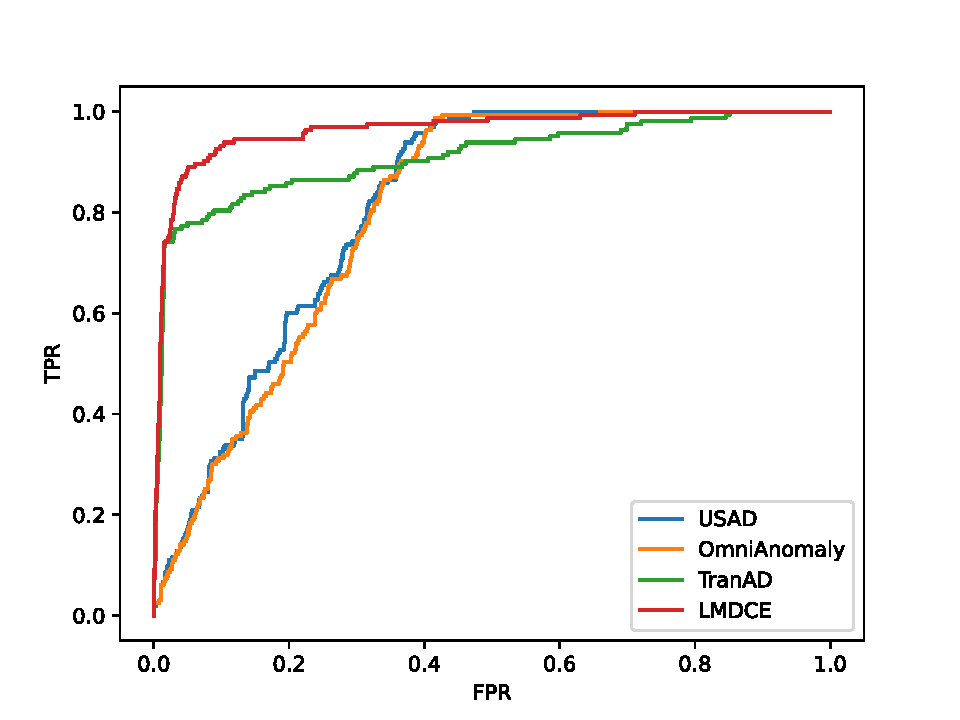
\includegraphics[width=1.00\textwidth]{Compare-ROC}
    \bicaption{\enspace USAD、OmniAnomaly、TranAD 和 LMDCE 的 ROC 曲线}{\enspace ROC curve of USAD, OmniAnomaly, TranAD and LMDCE}
    \label{fig:compare-roc}

\end{figure}

对于横向移动检测任务而言,ROC 曲线越靠左,说明模型在越低误报率的情况下可具有同样的检测性能;越靠上,说明在同样误报容忍度的情况下检测性能越高。从 ROC 曲线可以看出,LMDCE 在误报率低于 0.05 的情况下即具有显著优于 TranAD 和其他模型的检测性能,因此适用于横向移动检测任务。

\subsection{LMDCE 特征筛选}
\label{sec:feature-filter}

本小节利用第~\ref{sec:filter}~节的特征重要度评估结果,对流量特征进行筛选,以缩短 LMDCE 的训练时间,同时避免不相关的特征影响性能。通过实验,观察了从 2 个特征到 79 个特征之下,LMDCE 的训练时间和 AUC 分数的变化,如图~\ref{fig:experiment-filter}~所示。

\begin{figure}[t]
    \centering
    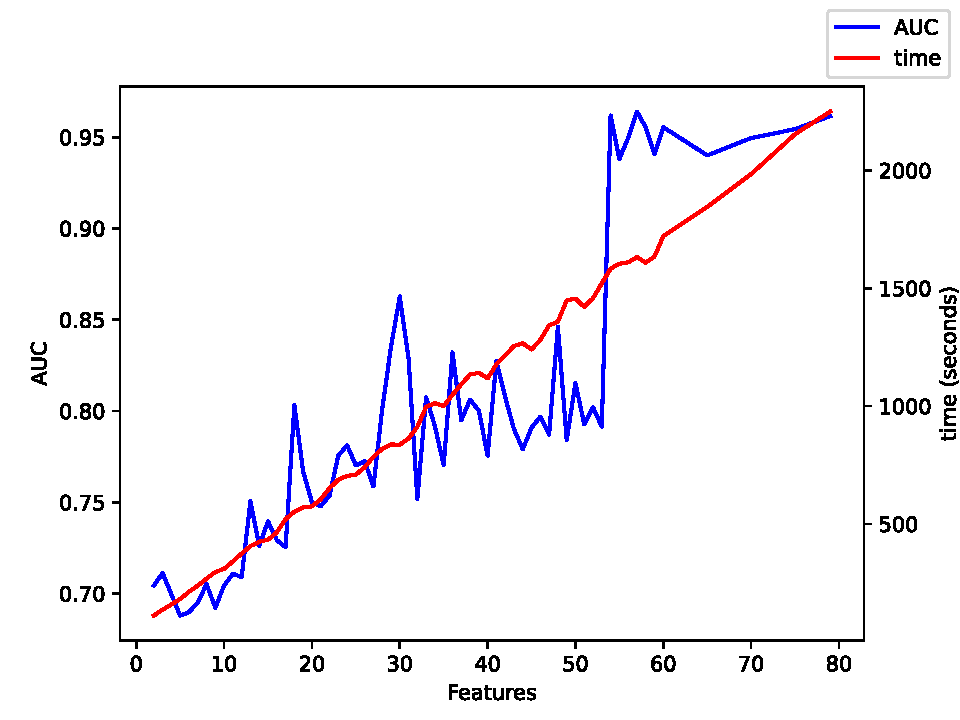
\includegraphics[width=1.00\textwidth]{filter}
    \bicaption{\enspace AUC 分数、训练时间与特征数量折线图}{\enspace Lineplot between AUC, training time and the number of features}
    \label{fig:experiment-filter}

\end{figure}

实验结果说明,在保留 57 个特征的情况下,LMDCE 达到最佳性能,AUC 分数达到 0.9640,同时训练时间可缩短 27\%;而在保留全量 79 个特征的情况下,AUC 分数为 0.9615。因此,本文验证了基于特征重要度评估的特征筛选的有效性,去除不相关的特征后,在缩短训练时间的同时提升了性能。

\subsection{LMDCE 消融实验}

为了研究 LMDCE 的每个组成部分的相对重要性,本文进行了消融实验,分别去除模型中的组成部分,并观察其对 AUC 分数的影响。首先,本文考虑了去除编码器—解码器的模型,即仅使用循环神经网络;其次,本文考虑了去除空间特征嵌入模块的模型,即仅输入网络流量的特征而不输入节点空间嵌入向量;第三,本文考虑了去除时间特征嵌入模块的模型,即使用恒等变换替换循环神经网络;第四,本文考虑了去除两步预测机制的模型,即直接采用 $O_{1,t}$ 作为预测值。实验结果如表~\ref{tab:experiment-ablation}~所示,对应的 ROC 曲线图如图~\ref{fig:experiment-ablation}~所示。

\begin{table}[t]
    \bicaption{\enspace LMDCE 消融实验结果}{\enspace Results of ablation experiments of LMDCE}
    \label{tab:experiment-ablation}
    \centering
    \footnotesize% fontsize
    \setlength{\tabcolsep}{4pt}% column separation
    \renewcommand{\arraystretch}{1.2}%row space 
    \begin{tabular}{lcccccccc}
        \hline
        消融部分 & AUC\\
        \hline
        编码器—解码器 & 0.79992\\
        空间特征嵌入模块 & 0.92614\\
        时间特征嵌入模块 & 0.93493\\
        两步预测机制 & 0.93797\\
        无 & 0.96401\\
        \hline
    \end{tabular}
\end{table}

\begin{figure}[t]
    \centering
    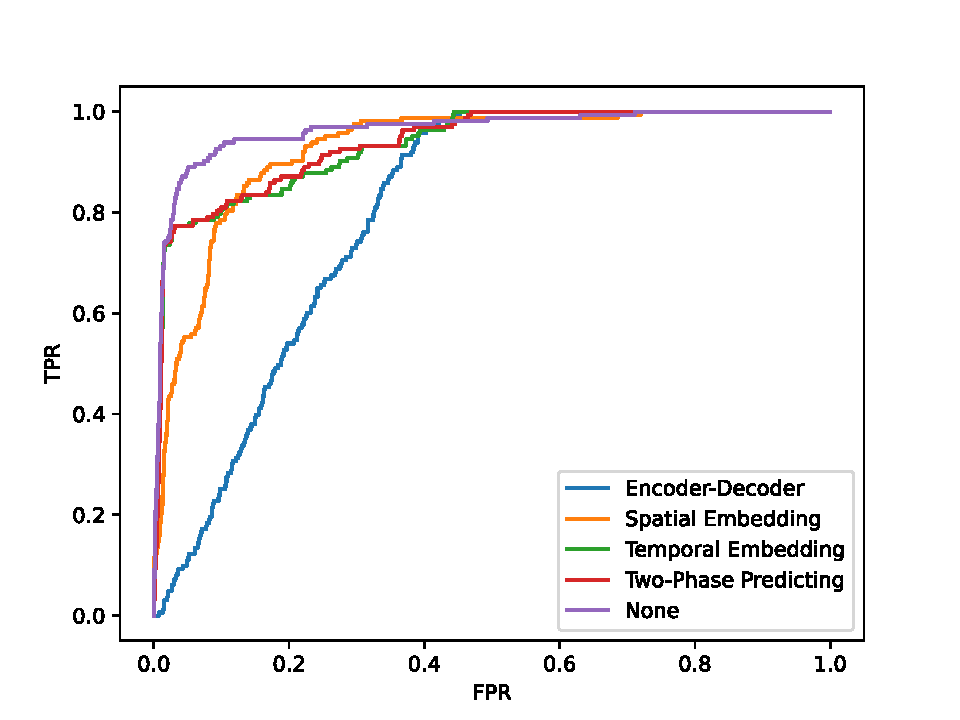
\includegraphics[width=1.00\textwidth]{ablation}
    \bicaption{\enspace 消融实验 ROC 曲线图}{\enspace ROC curve of ablation experiments}
    \label{fig:experiment-ablation}

\end{figure}

根据消融实验,可以得出以下结论:

\begin{itemize}
    \item 去除编码器—解码器结构之后,AUC 分数下降最大,并且 ROC 曲线整体右移,说明该结构在横向移动检测中起最重要的作用。
    \item 去除空间特征嵌入模块之后,AUC 分数下降了 0.04,并且 ROC 曲线稍有右移。在横向移动检测任务中,模型应在低误报率情况下保持尽可能高的检测率,也就是 ROC 曲线应尽可能靠左。因此,尽管其 AUC 分数达到了 0.92,但仍然容易产生警报泛滥。这说明,空间特征嵌入模块有助于减少模型的误报。
    \item 模型的时间特征嵌入模块和两步预测机制有助于进一步提高模型的检测率。分别去除这两个模块(机制)后,ROC 曲线没有右移,但有下移,这说明在误报率不变的情况下,模型的检测率有所提升。
\end{itemize}

% \subsection{网络流量的空间特征转换方法验证}

% 本节将对比不同的空间特征转换方法,将对 Node2vec、GCN、GraphSAGE、GAT 等方法进行对比,选出最佳的空间特征转换方法。实验结果如表~\ref{tab:experiment-gnn-result}~所示。其中,Node2Vec(global) 的窗口大小为 10,步长为 20,表示该模型将根据节点所在的整个节点群调整节点的嵌入向量;Node2vec(local) 的窗口大小为 2,步长为 4,表示该模型在调整嵌入向量时,将更关注节点的单跳或二跳邻居。

% \begin{table}[t]
%     \bicaption{\enspace 空间特征转换方法实验结果}{\enspace Results of Experiments Verifying Spacial Feature Transformations}
%     \label{tab:experiment-gnn-result}
%     \centering
%     \footnotesize% fontsize
%     \setlength{\tabcolsep}{4pt}% column separation
%     \renewcommand{\arraystretch}{1.2}%row space 
%     \begin{tabular}{lcccccccc}
%         \hline
%         组别 & AUC\\
%         \hline
%         Node2vec(global) & 0.95368\\
%         Node2vec(local) & 0.95536\\
%         GCN & 0.95884\\
%         GraphSAGE & 0.96192\\
%         GAT & 0.94764\\
%         None & 0.92614\\
%         \hline
%     \end{tabular}
% \end{table}

% 根据实验结果,可以看出,使用空间特征转换方法与不使用相比,可以显著提高模型的性能。在各种图神经网络模型中,GraphSAGE 的性能最佳,这是因为该模型的图卷积层同时考虑节点本身的信息和节点邻居的信息来生成节点的向量,而其他两个模型仅考虑节点邻居的信息。GAT 的性能较低,这可能是由于该模型需学习节点邻居的注意力参数导致。

% \subsection{网络流量的时间特征转换方法验证}

% 本节验证网络流量的时间特征转换方法,将 GRU、LSTM 与不使用循环神经网络模型进行对比。实验参数如表~\ref{tab:experiment-gru}~所示。

% \begin{table}[t]
%     \bicaption{\enspace 时间特征转换方法实验参数}{\enspace Parameters of Experiments Verifying Temporal Feature Transformations}
%     \label{tab:experiment-gru}
%     \centering
%     \footnotesize% fontsize
%     \setlength{\tabcolsep}{4pt}% column separation
%     \renewcommand{\arraystretch}{1.2}%row space 
%     \begin{tabular}{lcccccccc}
%         \hline
%         组别 & 模型 & 输入层维度 & 隐藏层维度 & 层数\\
%         \hline
%         GRU-1 & GRU & 145 & 145 & 1\\
%         GRU-3 & GRU & 145 & 145 & 3\\
%         LSTM-1 & LSTM & 145 & 145 & 1\\
%         LSTM-3 & LSTM & 145 & 145 & 3\\
%         None & & & & \\
%         \hline
%     \end{tabular}
% \end{table}

% 实验结果如表~\ref{tab:experiment-gru-result}~所示。

% \begin{table}[t]
%     \bicaption{\enspace 时间特征转换方法实验结果}{\enspace Results of Experiments Verifying Temporal Feature Transformations}
%     \label{tab:experiment-gru-result}
%     \centering
%     \footnotesize% fontsize
%     \setlength{\tabcolsep}{4pt}% column separation
%     \renewcommand{\arraystretch}{1.2}%row space 
%     \begin{tabular}{lcccccccc}
%         \hline
%         组别 & AUC\\
%         \hline
%         GRU-1 & 0.94417\\
%         GRU-3 & 0.95333\\
%         LSTM-1 & 0.94966\\
%         LSTM-3 & 0.95368\\
%         None & 0.93275\\
%         \hline
%     \end{tabular}
% \end{table}

% 根据实验结果,可以看出,与不使用时间特征转换方法相比,使用时间特征转换方法可以提高模型的性能。与 GRU 模型相比,采用 LSTM 模型的性能更高,其提升程度超过了采用多层模型所能提升的程度。在所有实验中,性能最高的是 LSTM-3 组。

% \subsection{横向移动检测模型的二阶段训练方法验证}

% 本节对横向移动检测模型的二阶段训练方法进行验证。实验包括两组,实验组去除二阶段训练方法,仅使用一阶段训练,模型结构图如图~\ref{fig:model-one-phase}~所示;对照组保留二阶段训练方法。实验结果如表~\ref{tab:experiment-phase-result}~所示。

% \begin{figure}[t]
%     \centering
%     \includegraphics[width=1.00\textwidth]{model-one-phase}
%     \bicaption{\enspace 去除二阶段训练方法的横向移动检测模型结构}{\enspace Lateral Movement Detection Model Without Two-phase Training}
%     \label{fig:model-one-phase}

% \end{figure}

% \begin{table}[t]
%     \bicaption{\enspace 横向移动检测模型的二阶段训练方法实验结果}{\enspace Results of Experiments Verifying Two-phase Training}
%     \label{tab:experiment-phase-result}
%     \centering
%     \footnotesize% fontsize
%     \setlength{\tabcolsep}{4pt}% column separation
%     \renewcommand{\arraystretch}{1.2}%row space 
%     \begin{tabular}{lcccccccc}
%         \hline
%         组别 & AUC\\
%         \hline
%         实验组 & 0.93966\\
%         对照组 & 0.95368\\
%         \hline
%     \end{tabular}
% \end{table}

% 根据实验结果,可以看出,与使用一阶段训练方法相比,采用二阶段训练方法,可以提高模型的性能。

\subsection{LMDCE 异常阈值选取}
\label{sec:threshold}

LMDCE 为每个流量 $X_i$ 给出了检测分数。在前面小节的实验中,本文主要通过 AUC 分数来对比模型的性能。然而,还需要以一定的手段确定检测分数的阈值,才能完成良性流量和横向移动流量的分类任务。

本文统计了不同阈值设定下的 TP、FP、TPR、FPR、精确率 和 F1 分数(关于这些指标的介绍见第~\ref{sec:kpi}~节),结果如表~\ref{tab:experiment-kpi}~所示。精确率、F1 分数随 TP 的变化如图~\ref{fig:experiment-kpi}~所示。

\begin{table}[t]
    \bicaption{\enspace 不同阈值设定下的 LMDCE 测试结果}{\enspace Results of LMDCE under different thresholds}
    \label{tab:experiment-kpi}
    \centering
    \footnotesize% fontsize
    \setlength{\tabcolsep}{4pt}% column separation
    \renewcommand{\arraystretch}{1.2}%row space 
    \begin{tabular}{ccccccccc}
        \hline
        TP & FP & TPR & FPR & 精确率 & F1 分数\\
        \hline
        120 & 119 & 0.7362 & 0.0151 & 0.5021 (\approx 1/2) & 0.5970\\
        138 & 265 & 0.8466 & 0.0337 & 0.3424 (\approx 1/3) & 0.4876\\
        145 & 402 & 0.8896 & 0.0511 & 0.2651 (\approx 1/4) & 0.4085\\
        \hline
    \end{tabular}
\end{table}

\begin{figure}[t]
    \centering
    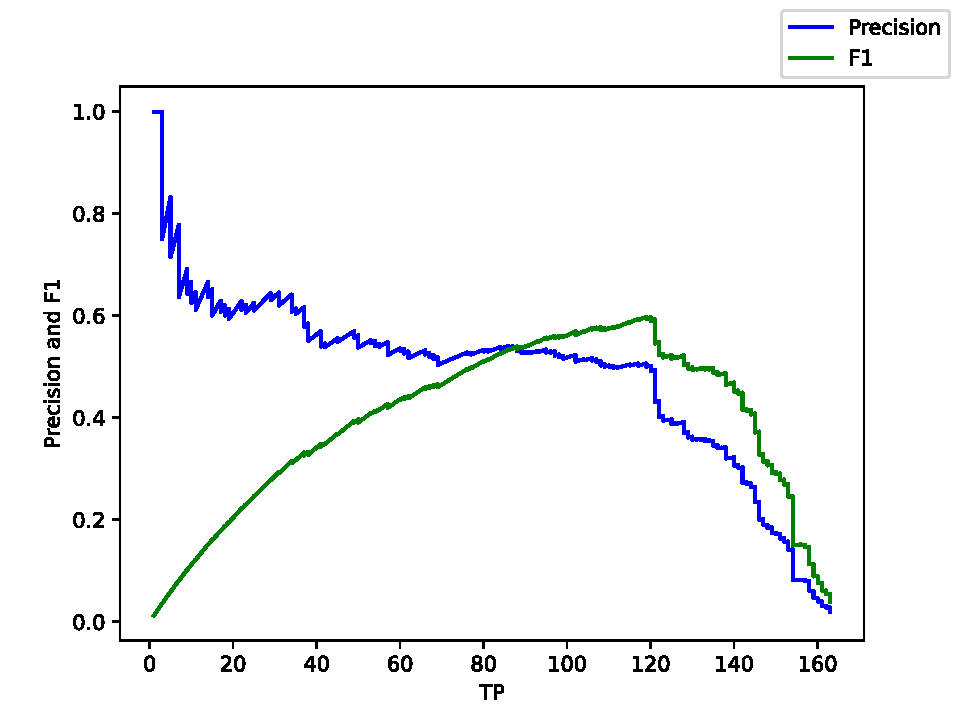
\includegraphics[width=1.00\textwidth]{kpi}
    \bicaption{\enspace 精确率、F1 分数随 TP 的变化曲线图}{\enspace Lineplot of precision and F1 score with TP}
    \label{fig:experiment-kpi}

\end{figure}

由于本文提出的横向移动检测任务是针对每条流量进行检测,而一次横向移动行为对应上百条流量,因此,实际上不需要达到很高的检测率即可达到检测效果,只需检测大部分流量即可。本文推荐采取精确率大约为二分之一所对应的阈值,此时检出的流量中,有大约一半为横向移动流量,检测率为 73.6\%,误报率为 1.5\%,达到了检测率与误报率之间的平衡。另一方面,若对误报率的容忍较高,则可把精确率放宽至大约四分之一,此时检测率可达到大约 89\%,误报率为 5\%。

\subsection{两阶段方法集成验证}

本文提出的横向移动检测方法分为两个阶段,第~\ref{sec:verify-1}~节和第~\ref{sec:verify-2}~-~\ref{sec:threshold}~节分别对两个阶段进行了验证。本小节对两个阶段进行集成验证。

在第~\ref{sec:verify-1}~节中,本文检测到了 8 条关键横向移动流量。在第~\ref{sec:verify-2}~节中,本文对测试集中的所有流量给出了评估分数。这 8 条流量对应的 LMDCE 以及其他方法的评估分数在测试集中的排名如表~\ref{tab:experiment-rank}~所示。

\begin{table}[t]
    \bicaption{\enspace 关键横向移动流量的评估分数排名}{\enspace Ranks of key lateral movement flows}
    \label{tab:experiment-rank}
    \centering
    \footnotesize% fontsize
    \setlength{\tabcolsep}{4pt}% column separation
    \renewcommand{\arraystretch}{1.2}%row space 
    \begin{tabular}{ccccccccc}
        \hline
        源 IP 地址 & 源端口 & 目的 IP 地址 & 目的端口 & LMDCE & USAD & OmniAnomaly & TranAD\\
        \hline
        10.16.0.45 & 52906 & 144.122.71.18 & 6443 & 1 & 1 & 2422 & 1\\
        10.16.0.45 & 47002 & 144.122.71.18 & 6443 & 18 & 2694 & 808 & 114\\
        10.16.0.45 & 59624 & 95.179.254.105 & 443 & 53 & 439 & 371 & 219\\
        10.16.0.45 & 45956 & 144.122.71.18 & 6443 & 110 & 1251 & 3 & 56\\
        10.16.0.45 & 46988 & 144.122.71.18 & 6443 & 151 & 2859 & 2766 & 150\\
        10.16.0.45 & 54902 & 144.122.71.36 & 9001 & 271 & 900 & 1856 & 1833\\
        10.16.0.45 & 52904 & 144.122.71.18 & 6443 & 326 & 1160 & 2 & 3701\\
        144.122.71.36 & 9001 & 10.16.0.45 & 48754 & 636 & 2606 & 44 & 3196\\
        \hline
    \end{tabular}
\end{table}

根据第~\ref{sec:threshold}~节中的阈值分析,如果仅使用 LMDCE ,即使忍受了 1/4 的精确率,也仅能检出 145 条横向移动流量,而在 8 条关键横向移动流量中仅有 4 条排名在 145 以内。若使用 USAD、OmniAnomaly、TranAD 方法,分别仅有 1、3、3 条横向移动流量排名在 145 以内,并且根据第~\ref{sec:verify-2}~节的实验结果,这些方法的精确率更低。因此,不论是仅使用第二阶段的颊侧方法,还是采用现有的其他方案,均不能有效检出关键的横向移动流量。特别是,负载(10.16.0.45)与外部服务器(144.122.71.36:9001)通信的流量会被排除在外,导致无法找到攻击者所使用的服务器。

造成这种现象的原因是,LMDCE 基于自注意力机制实现,其在检测时间特性上有优势,而不擅长于捕获图的空间关系。

因此,尽管第一阶段的方法实现简单,检出的流量也较少,但仍是方法不可或缺的一部分,因为该方法检出的都是十分重要的、代表关键横向移动行为的流量,从而本文验证了两阶段集成方法的有效性。

\section{本章小结}

本章提出了基于 Transformer 的两阶段横向移动检测方法,达到了研究目标。通过基于最值和拓扑的横向移动检测,本文检出了 8 条横向移动流量,这些流量代表了关键的横向移动行为,即攻击者利用了入侵后的节点,对 API 服务器进行非法通信。通过基于 Transformer 的横向移动检测模型 LMDCE,本文达到了 96.4\% 的 AUC 分数,优于其他现有的模型。通过特征筛选,本文节省了 27\% 的训练时间,并使模型达到了最佳性能。本文进行了消融实验,验证了 LMDCE 各模块的相对重要性。本文还讨论了 LMDCE 的异常阈值选取。最后,本文对方法的两个阶段做了集成分析。

}